
\begin{figure}%
	\centering%
	\caption{Histogram of Stock Prices}%
	\label{fig:histogram_prices}%
	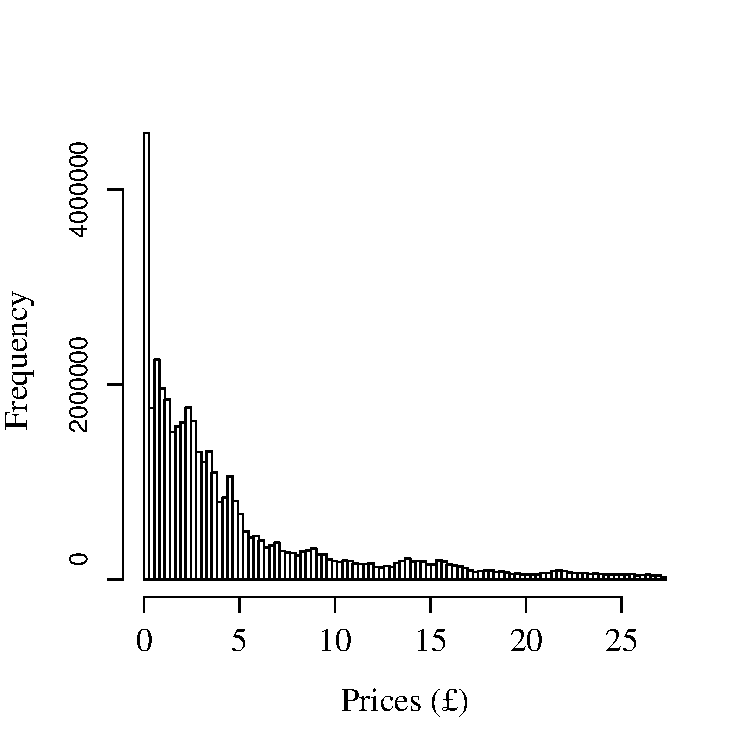
\includegraphics[width=.6\textwidth]{figures/prices_hist_login_days.pdf}
	\fignote{Figure shows the histogram of prices on login days. Outliers in the 99 percentile are excluded.}
\end{figure}

\clearpage

\begin{figure}[hbt!]
	\caption{Leftmost Stock Price Digit and Probability of Sale \\ Prices Increasing Sample by Price Range}%
	\label{fig:left_digit_sell_increase}%
	\centering%	
	\bigskip
	\subfigure[Price = \pounds0.11 to \pounds1.01]{
		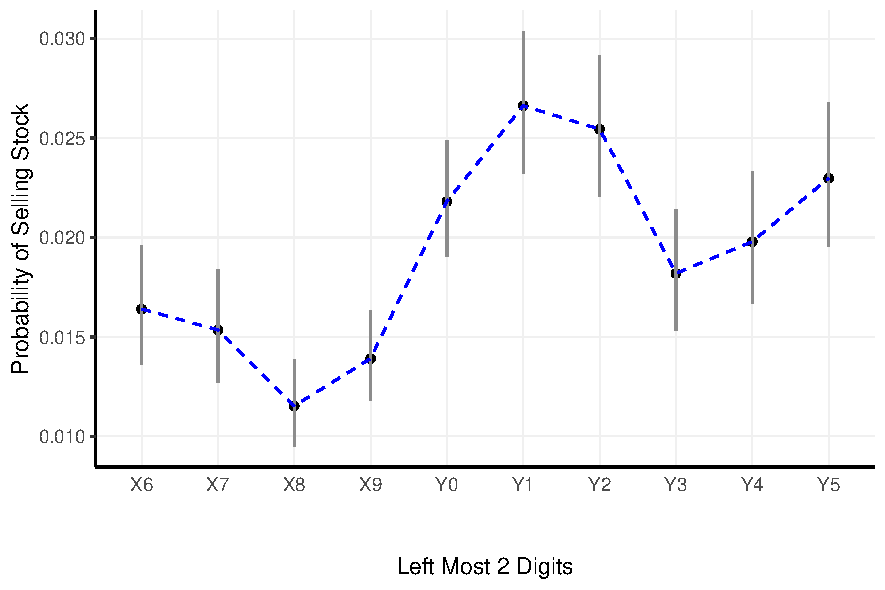
\includegraphics[width=0.45\textwidth]{figures/Left2increases_1pbin_CI.pdf}
		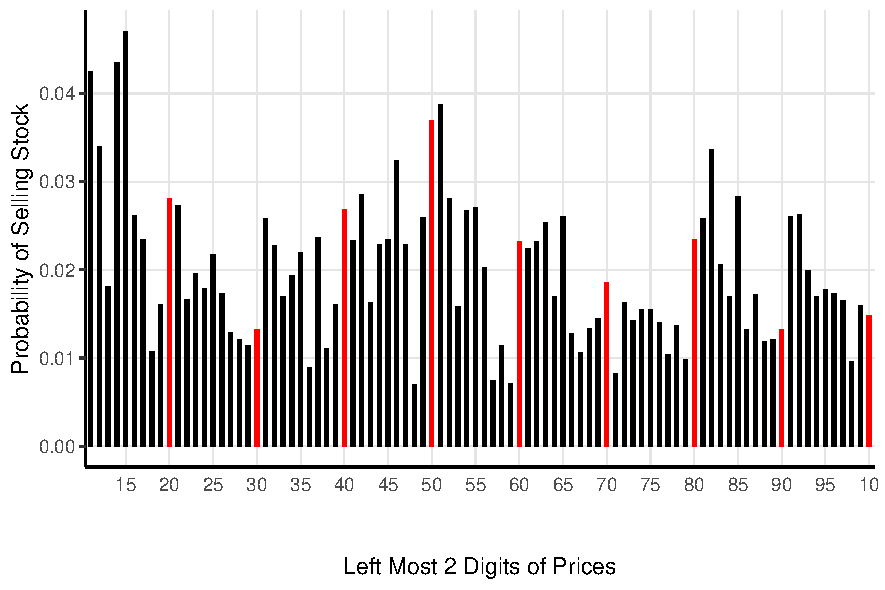
\includegraphics[width=0.45\textwidth]{figures/2left_increase_bin1p.pdf}
	}
	\subfigure[Price = \pounds1.01 to \pounds10.1]{
		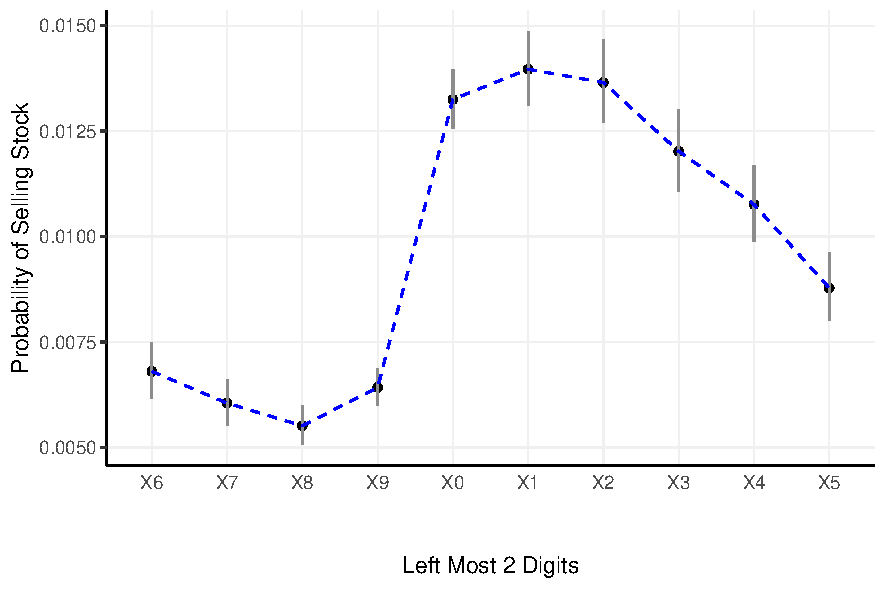
\includegraphics[width=0.45\textwidth]{figures/Left2increases_10pbin_CI.pdf}
		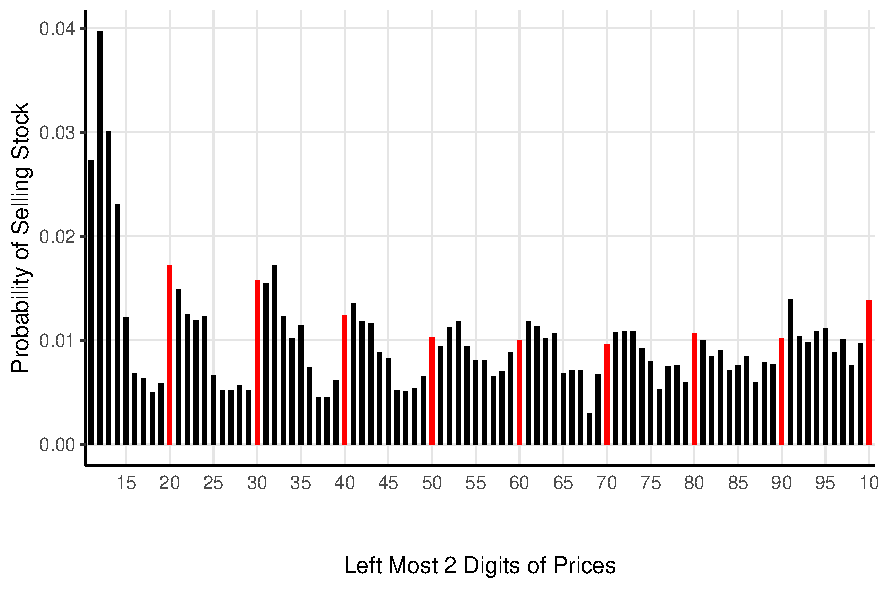
\includegraphics[width=0.45\textwidth]{figures/2left_increase_bin10p.pdf}
	}
	\subfigure[Price = \pounds11 to \pounds101]{
		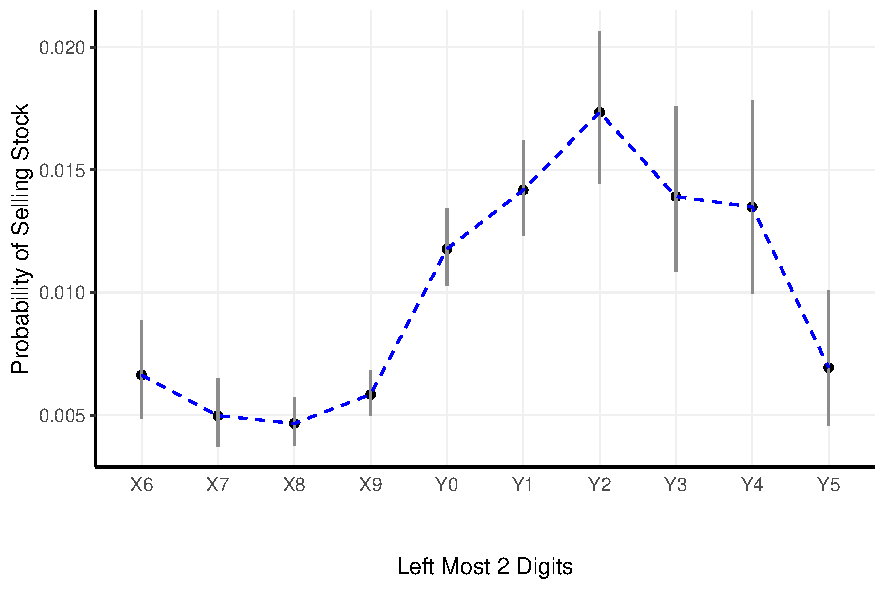
\includegraphics[width=0.45\textwidth]{figures/Left2increases_1poundbin_CI.pdf}
		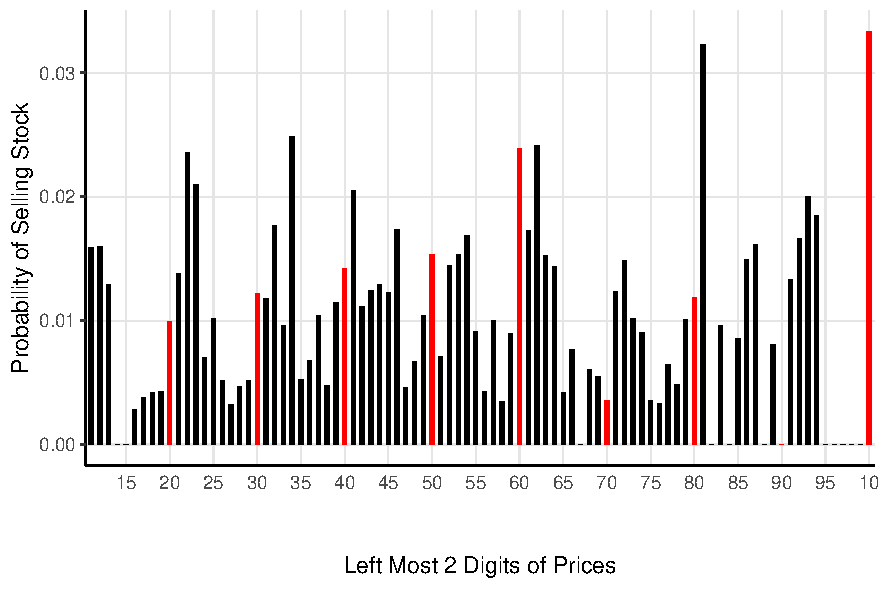
\includegraphics[width=0.45\textwidth]{figures/2left_increase_bin1pound.pdf}
	}
	\fignote{£$Y$ in the X-axes is equivalent to £$X+1$ (e.g., £X9 could include £0.19, £1.9, £19, etc., while £Y0 could include £0.20, £2.0, £20, etc.). Panels A, B and C show equal size bins of 1p, 10p and £1, respectively. Panel A corresponds to 26.22\% of the observations in the prices increasing sample; Panel B, to 49.28\%; and Panel C, to 8.03\%.}
\end{figure}

\begin{figure}[hbt!]
	\caption{Leftmost Stock Price Digit and Probability of Sale \\ Prices Decreasing Sample by Price Range}%
	\label{fig:left_digit_sell_decrease}%
	\centering%	
	\bigskip
	\subfigure[Price = \pounds0.10 to \pounds1.00]{
		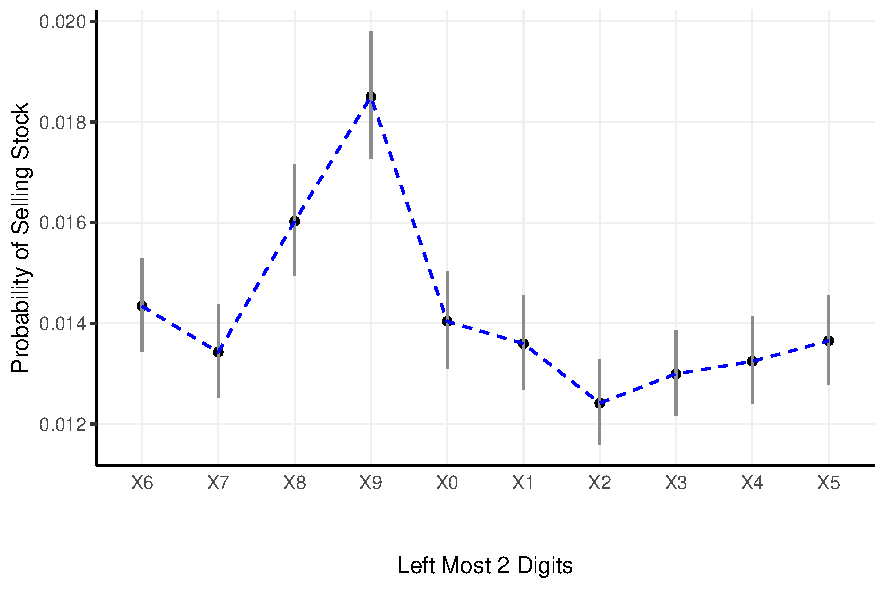
\includegraphics[width=0.45\textwidth]{figures/Left2decreases_1pbin_CI.pdf}
		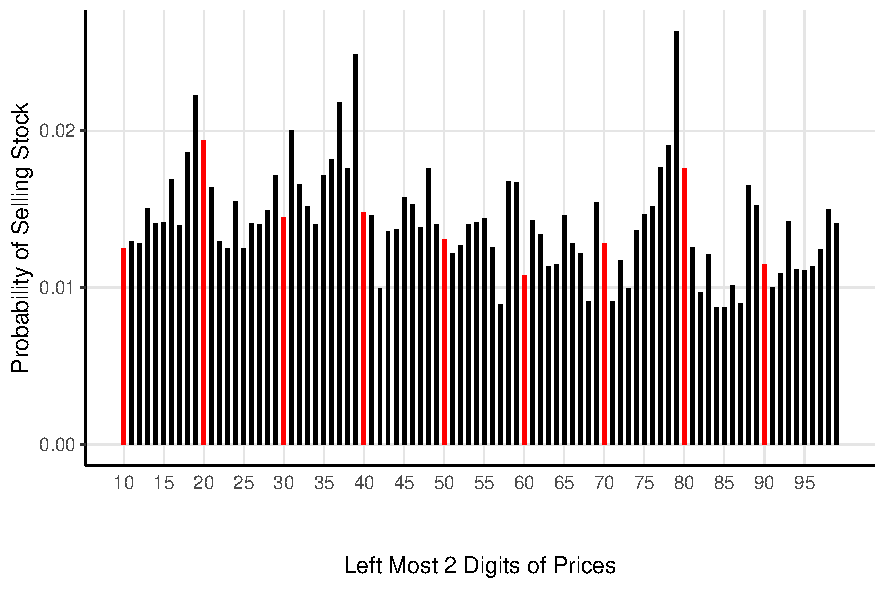
\includegraphics[width=0.45\textwidth]{figures/2left_decrease_bin1p.pdf}
	}
	\subfigure[Price = \pounds1.00 to \pounds10.0]{
		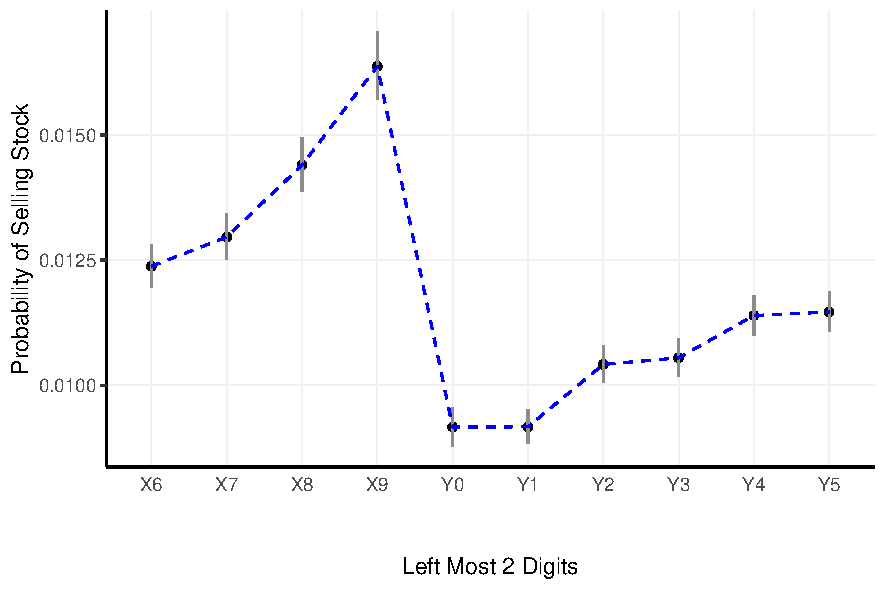
\includegraphics[width=0.45\textwidth]{figures/Left2decreases_10pbin_CI.pdf}
		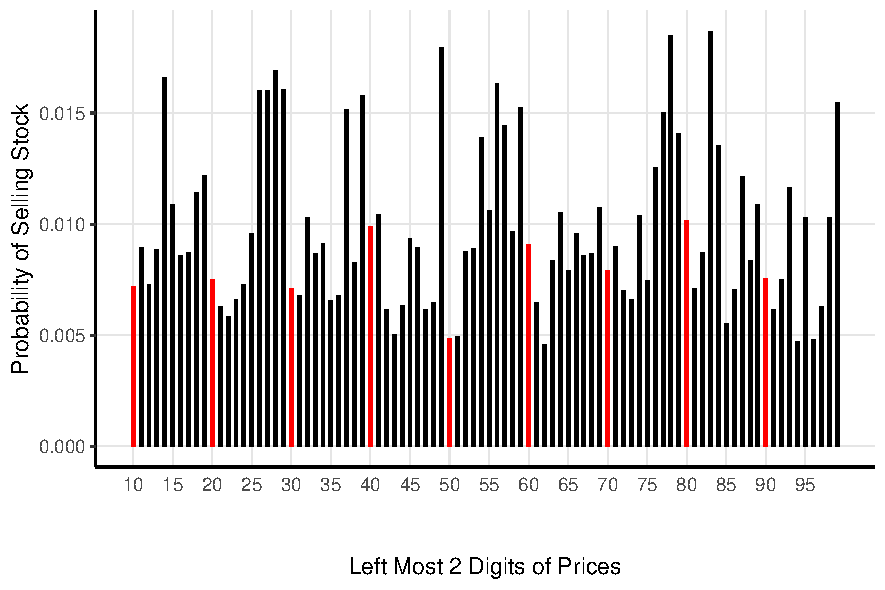
\includegraphics[width=0.45\textwidth]{figures/2left_decrease_bin10p.pdf}
	}
	\subfigure[Price = \pounds10 to \pounds100]{
		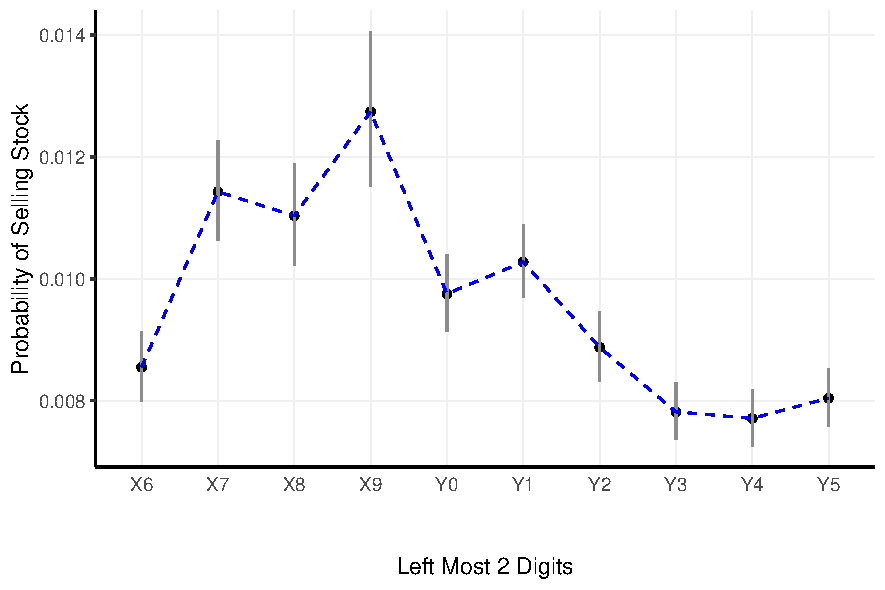
\includegraphics[width=0.45\textwidth]{figures/Left2decreases_1poundbin_CI.pdf}
		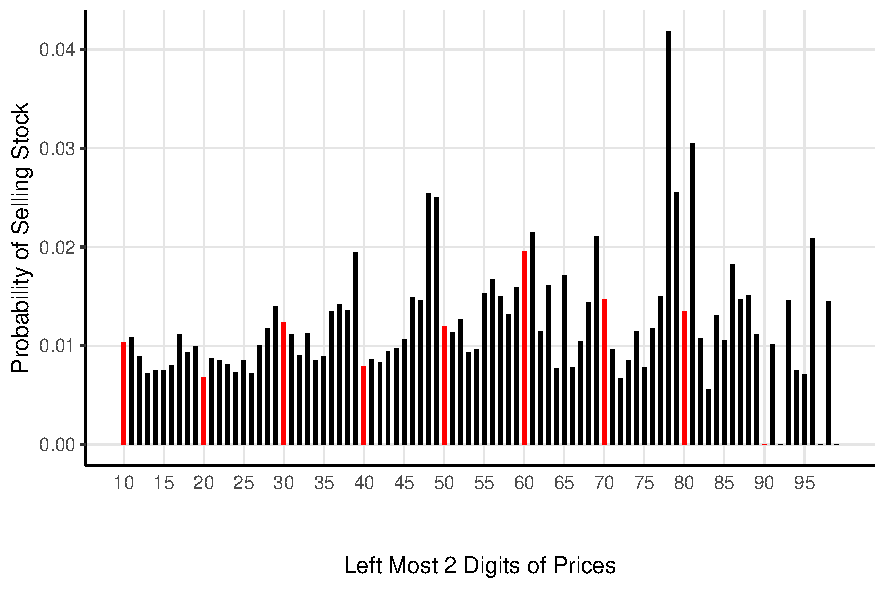
\includegraphics[width=0.45\textwidth]{figures/2left_decrease_bin1pound.pdf}
	}
	\fignote{£$Y$ in the X-axes is equivalent to £$X+1$ (e.g., £X9 could include £0.19, £1.9, £19, etc., while £Y0 could include £0.20, £2.0, £20, etc.). Panels A, B and C show equal size bins of 1p, 10p and £1, respectively. Panel A corresponds to 25.89\% of the observations in the prices decreasing sample; Panel B, to 41.15\%; and Panel C, to 6.74\%.}
\end{figure}

\clearpage

\begin{figure}[hbt!]
	\caption{Sample Selection and Simulation Exercise}%
	\label{fig:sample_selection_test}%
	\centering%	
	\bigskip
	\subfigure[Price Increasing Sample]{
		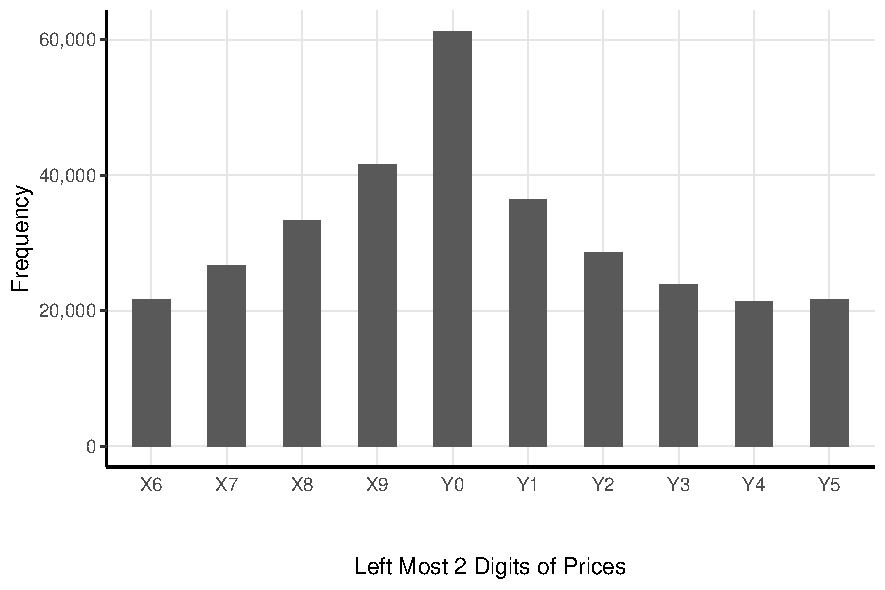
\includegraphics[width=0.45\textwidth]{figures/left2_second_increase_count.pdf}
		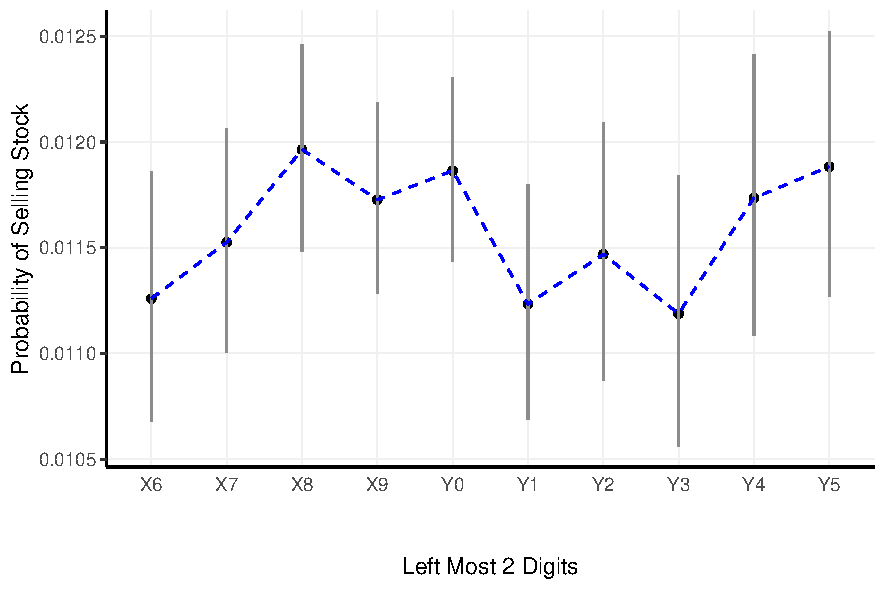
\includegraphics[width=0.45\textwidth]{figures/Left2increase_probCI_random_sell.pdf}
	}
	\subfigure[Price Decreasing Sample]{
	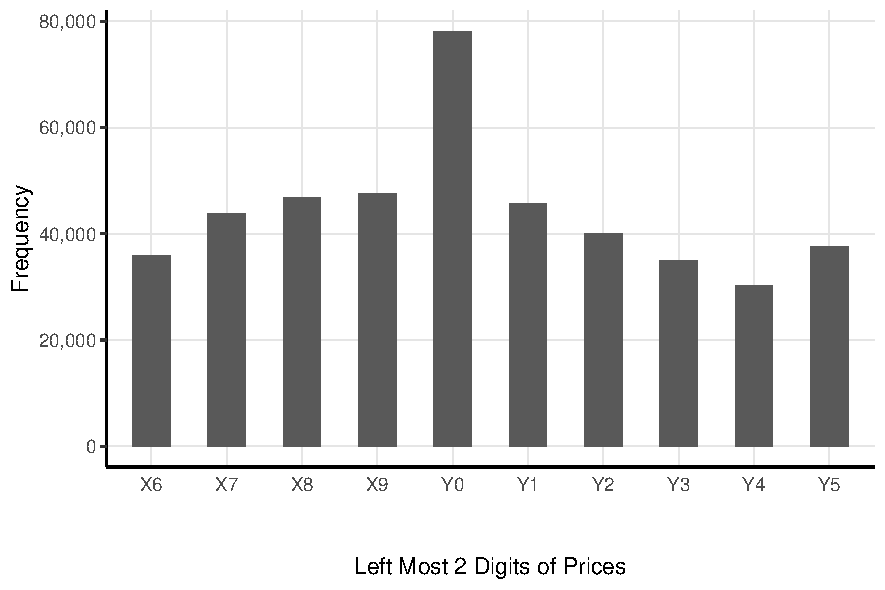
\includegraphics[width=0.45\textwidth]{figures/left2_second_decrease_count.pdf}
	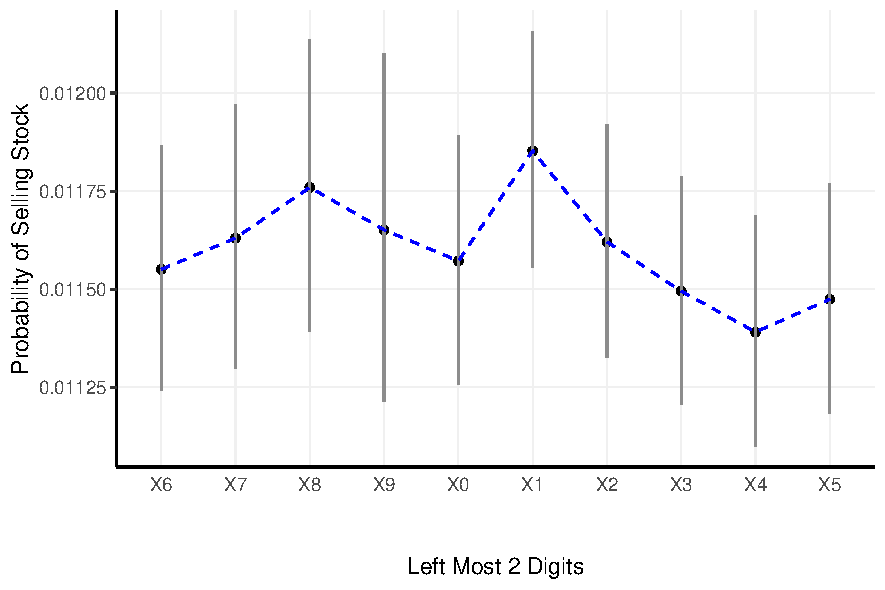
\includegraphics[width=0.45\textwidth]{figures/Left2decrease_probCI_random_sell.pdf}
}
\end{figure}


\begin{figure}[hbt!]
	\caption{Leftmost Stock Price Digit and Probability of Sale, Sell Days \textcolor{blue}{[EQ: sell days results at here the end of the Appendix. But perhaps they should go before Figure A4?]}}%
	\label{fig:left_digit_sell}%
	\centering%	
	\bigskip
	\subfigure[Price Increasing]{
		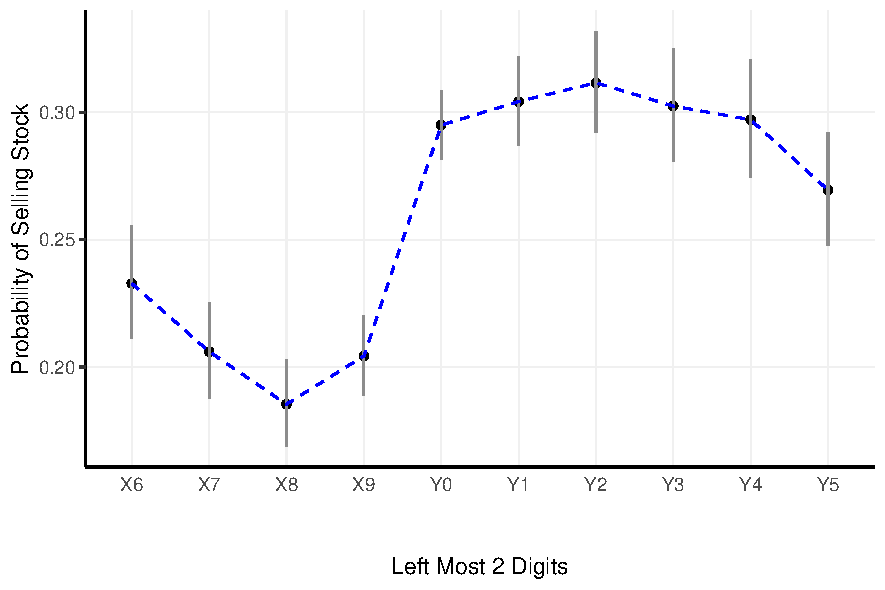
\includegraphics[width=0.45\textwidth]{figures/Left2increase_probCI2_sell_sample.pdf}
		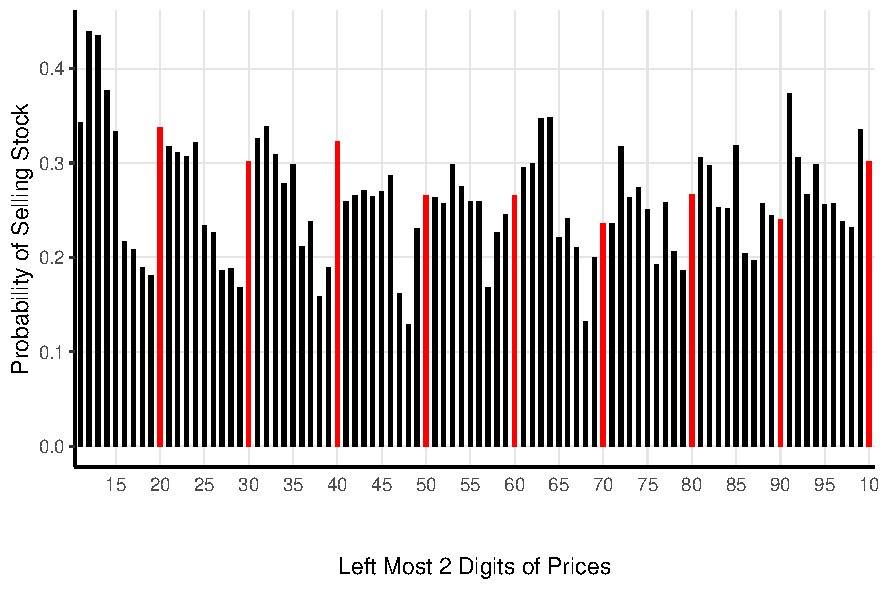
\includegraphics[width=0.45\textwidth]{figures/2left_increase2_sell_sample.pdf}	
	}
	\subfigure[Price Decreasing]{
		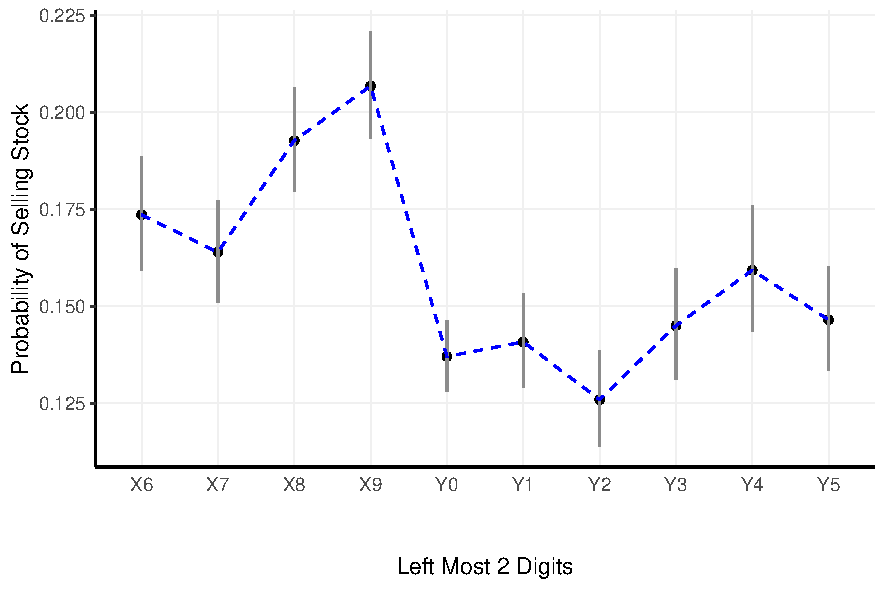
\includegraphics[width=0.45\textwidth]{figures/Left2decrease_probCI2_sell_sample.pdf}
		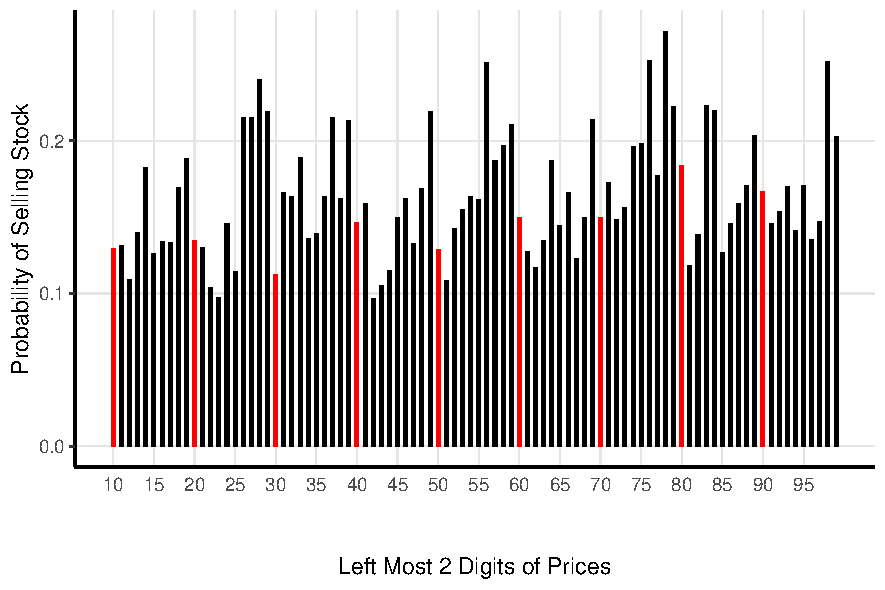
\includegraphics[width=0.45\textwidth]{figures/2left_decrease2_sell_sample.pdf}	
	}
	\fignote{£$Y$ in the X-axes is equivalent to £$X+1$ (e.g., £X9 could include £0.19, £1.9, £19, etc., while £Y0 could include £0.20, £2.0, £20, etc.).}
\end{figure}



\begin{figure}[hbt!]
	\caption{Probability of Topping-up \textcolor{blue}{[EQ: I remember we talked with George about doing the topping up analysis. Perhaps we could just tell him that the analysis did not work and drop this plot? What do you think? Just in case, I am leaving the plots here for now. ]}}%
	\label{fig:topup}%
	\centering%	
	\bigskip
	\subfigure[Price Increasing Sample]{
		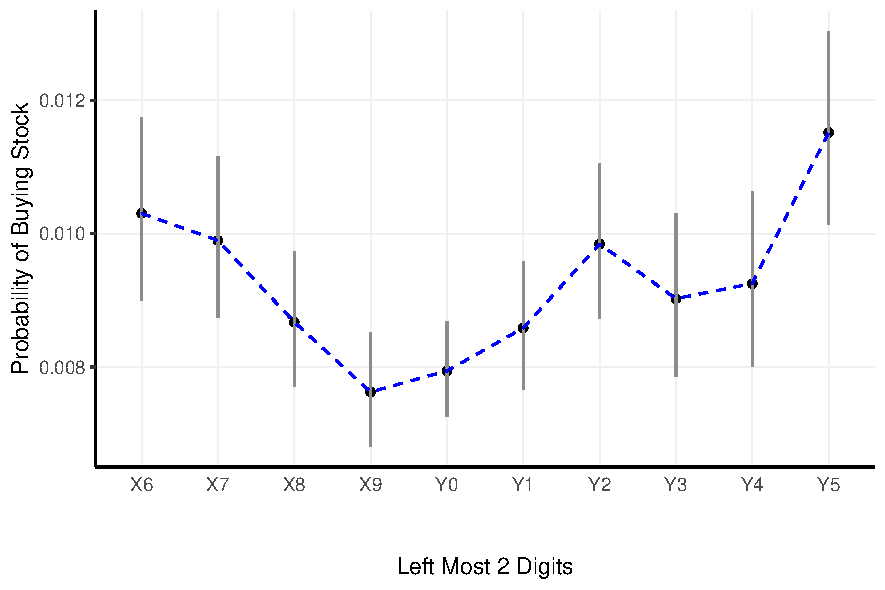
\includegraphics[width=0.70\textwidth]{figures/Left2increase_probCI_top_up.pdf}
	}
	\subfigure[Price Decreasing Sample]{

	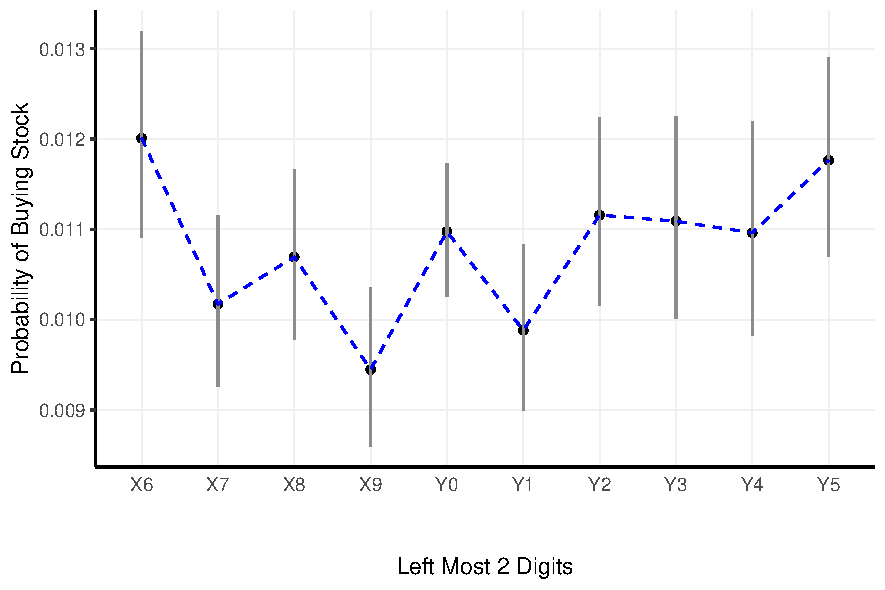
\includegraphics[width=0.70\textwidth]{figures/Left2decrease_probCI_top_up.pdf}
}
	\fignote{Figure shows the probability of topping up (increasing position in an stock) under the same sample selection. 	£$Y$ in the X-axes is equivalent to £$X+1$ (e.g., £X9 could include £0.19, £1.9, £19, etc., while £Y0 could include £0.20, £2.0, £20, etc., ).}
\end{figure}


